\documentclass{scrartcl}
\usepackage[utf8]{inputenc}
\usepackage[english]{babel} % Trennung nach der neuen deutschen Rechtschreibung
\usepackage[utf8]{inputenc}
\usepackage{esint}
\usepackage[T1]{fontenc}
\usepackage{lmodern}
\usepackage{subcaption}
\usepackage{chemformula}
\usepackage{placeins}
\usepackage{multirow}
\usepackage{enumitem}
\usepackage{amssymb}
\usepackage{amsmath} % Erweiterte Mathematik-Umgebung
\usepackage{amsfonts} % zusätzliche Mathematik-Schrifttypen (v.a. \mathbb für Mengen)
\usepackage{ulem}
\usepackage{amsthm}
\usepackage{graphics}%soll beim Graphiken einfügen hilfreich sein
\usepackage{graphicx}
\usepackage{wrapfig}%lässt Textumflossene Bildeinbindung zu
\usepackage{epstopdf}%soll eps in pdf umwandeln
\usepackage{placeins}
\usepackage{amsthm}
\usepackage{subcaption}
\usepackage{wrapfig}
\usepackage{float}
\usepackage{hyperref}
\usepackage{ragged2e}

\usepackage[a4paper, portrait, margin=2.5cm]{geometry}

\setlength\parindent{0pt}

\begin{document}

\begin{titlepage}
    \begin{center}
        \vspace*{1cm}
        \Huge
        \textbf{Magnetic properties of atoms}
        
        \vspace{0.5cm}
        \LARGE
        \textit{PART II: Zeeman effect}
        
        \vspace{0.5cm}
        \LARGE
        Advanced Lab Course
        
        \vspace{1.5cm}
        \textbf{Louis-Hendrik Barboutie (020157041C), Frederik Ehl (0201719742) and Florence Schmerber (0201845640)}
        
        \vspace{1cm}
        Supervisor: Evelyn Pratami SINAGA
        \vfill
        

        \includegraphics[width=0.4\textwidth]{logo_uni.jpg}
        
        \Large
        $28^{\underline{\text{th}}}$ April 2022
    \end{center}
\end{titlepage}

\section{Introduction}

In this lab course we will study two effects in atomic physics: The Zeeman effect and electron spin resonance. The Zeeman effect, named after the physicist Pieter Zeeman in 1896,  is the splitting of atomic energy levels and can be seen if an atom is introduced to a magnetic field. There are different kinds of effects, but the one we will be interested today is the so called normal Zeeman effect on a cadmium lamp. This effect has various applications such as nuclear magnetic resonance spectroscopy or electron spin resonance spectroscopy \cite{Zeeman}, which we will also discover in this lab class. Through the study of the spectral lines, we can experimentally determine the Bohr magneton.\\
Electron spin resonance (ERS) is a method of spectroscopy to observe the behavior of unpaired electrons. First, we will measure the absorption of electromagnetic radiation then we will focus on the ERS experiment.
%ERS erweitern/besser erklären was wir machen.

\section{Theory}
\subsection{Zeeman effect}
If a charged particle like an electron is rotating in a circular path, the it has a magnetic moment $\Vec{\mu}$. In fact, there is a proportinal relation between the magnetic moment and the angular momentum $\Vec{L}$ given by:
\[ \Vec{\mu} = \frac{q}{2m}\Vec{L} \]
Now if this electron is introduced in a strong external magnetic field, then there will be an interaction between this field and the magnetic moment, causing the splitting of individual emission lines and thus energy levels.
%The emission lines of a material can usually be clearly separated. If the emitting material is placed in a strong magnetic field however, the individual emission lines are split up and instead of a single wavelength, several wavelength can now be observed. 
This phenomenon is called the Zeeman effect. In transitions of atomic states, where the total spin S is equal to zero, so called singlet states, and the total angular momentum of a state: $\Vec{J}=\Vec{L}+\Vec{S}$ is thus reduced to the orbital angular momentum $\Vec{L}$, we speak of the so called normal Zeeman effect. From the expression of the magnetic moment of the atom:
\[\Vec{\mu_J}=-\frac{g_J\mu_B}{\hbar}\Vec{J}\]
where $\mu_B$ is the Bohr magneton given by $\mu_B=\frac{\hbar e}{2m_e}$ and $g_J$ the Landé g-factor. For $\Vec{S} = 0$, the Landé factor takes the value of 1. We then can derive the overall energy levels of the splitting energies:
\begin{equation}
    U_Z = - m \mu_B B
\end{equation}
If there is no magnetic field, then the energy only depends on the principle quantum number n, which means there is no dependency of the magnetic quantum number m, which produces $2l +1$ degeneracy. That means each l and corresponding m will have the same energy. This is not the case if the magnetic moment isn't 0. Then the degeneracy is cancelled and the energies levels are slit according the the different m values (see equation 1).\\
The normal Zeeman effect can be observed on the photo electrons of cadmium, where the red emission line ($\lambda_0=643.8 $ nm) splits into three different lines with the energies corresponding to the three different possible values for $m_z: \pm1, 0$.
\begin{equation}
    \delta \lambda \approx \frac{\lambda^2}{2d\sqrt{n^2-1}}\frac{\delta \alpha}{\Delta \alpha}
    \label{equation_delta_lambda}
\end{equation}
\textit{How we derive this equation is shown in the appendix}\\ 
Here, $\Delta \alpha$ corresponds to half the length of the distance between the ring of first and the third interference order. On the other hand, $\delta \alpha$ is half of the length between the first and the third ring of the second interference order. The illustration of figure \ref{fig:delta_alpha} depicts these lengths.

\subsection{Induction}
Magnetic fields and electric currents are closely coupled, and one can give rise to the other and vice-versa. If for example an electrical conductor is put in a strong enough magnetic field, then the phenomenon of induction can occur. Electromagnetic induction is the process of generating a electric current with a magnetic field. For a wire loop, this is stated by Faraday's law of induction: \begin{equation}
    \mathcal{E} = - \frac{d \Phi_B}{dt}
    \label{gaußmag}
\end{equation} Where $\mathcal{E}$ is the electromotive force induced in the wire, and $\Phi_B$ is the magnetic flux where the loop is at. The magnetic flux is given by the Gauß law for magnetism: \begin{equation}
    \Phi_B = \oiint_{\partial S} \Vec{B}(t) \cdot d\Vec{S} 
\end{equation} Where $\Vec{S}$ is the oriented surface of the loop, and $\Vec{B}$ the magnetic field on that surface.

A coil can be seen as many wire loops stacked, and induction still occurs. The reverse effect is also true: if a current goes through a coil, it produces a magnetic field. If the current going through the coil is time-dependent, e.g. alternating current, the magnetic field produced will also be time-dependent. 

A coil put in a time-dependent magnetic field will have induced current flowing through it, as stated by Gauß' law in eq.~\ref{gaußmag}. When the magnetic field is produced by another coil, the voltages in both coils are linked: we talk about the induced voltage and absorbed voltage. If the current producing the magnetic field is alternating with a certain constant frequency, then there also exist a resonance frequency, where the induced voltage is maximum, and the absorbed voltage is minimum, ie. the "transfer of energy" is the most efficient.

\subsection{Electron spin resonance}
The magnetic moment associated with the spin can also interact with an external magnetic field. It can either orient itself parallel ($m_s = +\frac{1}{2}$) or antiparallel ($m_s = -\frac{1}{2}$) to the field. Here the potential energy will be:
\begin{equation}
    U_s = \pm \frac{1}{2}g_s\mu_s|B_0|
\end{equation}
In this case the energy is split according to the spin of the electron. The difference of energy levels is the absorption energy for an unpaired electron and is given by:
\begin{equation}
    \Delta E = g_s\mu_B|B_0| = h\nu
\end{equation}
The value for $B_0$ is given by the following equation:
\begin{equation*}
    B_0 = \mu_0 \cdot \left(\frac{4}{5}\right)^{\frac{3}{2}} \cdot \frac{n}{r} \cdot I
    \end{equation*}
With $\mu_0 = 4\pi \cdot 10^{-7} Vs/Am$, n = 320 and radius of the Hemlholtz coil being 6.8 cm.\\
The electron spin resonance is thus a phenomenon where an electron can change its spin orientation at a certain resonance frequency, which is given by:
\begin{equation}
    f = \frac{\Delta E}{h} = \frac{g_s\mu_BB}{h}
\end{equation}

\newpage

\section{Experimental Setup and procedure}
\begin{wrapfigure}{r}{5cm}
    \centering
    \includegraphics[width=0.25\textwidth]{bilder/interference.pdf}
    \caption{Interference orders}
    \label{fig:delta_alpha}
\end{wrapfigure}
The Cadmium lamp is placed in between two electromagnets, creating the slipping of the energy levels. The light from the lamp passes several lenses that are used to create the interference patterns that we can see afterwards and analyze. Finally the light passes through a red filter, since we want to analyze the Zeeman effect for red light.\\
As the intensity of the magnetic field depends on the applied current, a calibration curve with the relation between the applied current and the resulting magnetic field is needed. Then, to determine the Bohr magneton $\mu_B$ , the value for $\Delta \alpha$ and $\delta \alpha$ have to be recorded (see figure \ref{fig:delta_alpha}) for different currents. The data can then be plugged into equation 2, with which the total energy can be calculated. The data is then plotted and the resulting slope corresponds to $-\mu_B$.\\
Finally, we analyze the behaviour of the interference pattern when the light from the Cadmium lamp passes two polarizers.
\begin{figure}[H]
    \centering
    \includegraphics[width=0.7\textwidth]{bilder/1652041363921.jpg}
    \caption{Experimental setup for the Zeeman effect experiment}
    \label{fig:Zeeman_setup}
\end{figure}

\section{Results and discussion}
The light emmited from the cadmium lamp is $\lambda = 643.8$ nm, the refractive index of glass is $n=1.4567$, and the thickness of the employed Fabry-Pérot etalon is $d=4.04$ mm.

\begin{equation}
    E_{total} = \frac{hc}{\lambda +\delta \lambda}
\end{equation}

We measure the $B$-field produced by the setup for the current $I$ going through the coils. Fitting our data with a slope fit, we obtain a relationship which allows us to transform from $I$ to $B$. We obtain a linear fit of the form $B = aI+b$.

\begin{figure}[h!]
    \centering
    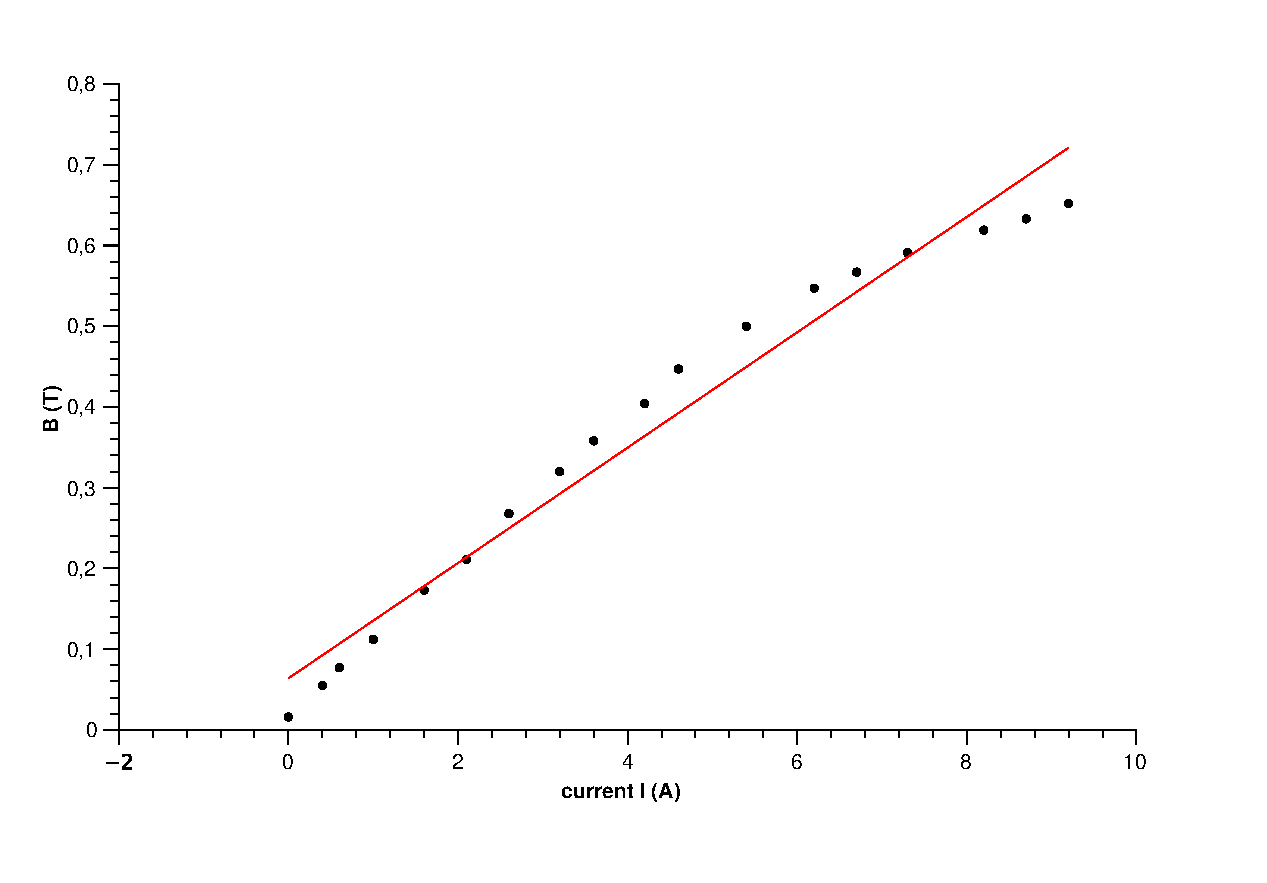
\includegraphics[width=0.7\textwidth]{B_function_I.eps}
    \caption{Magnetic field B as a function of the current I}
    \label{fig:B(I)}
\end{figure}


With our setup, we record the values of $2 \Delta \alpha$ and of $2 \delta \alpha$ as a function of the voltage and current.
% insert table here of data I, delta alpha, Delta alpha
\begin{table}[!ht]
    \centering
    \begin{tabular}{c|c|c|c}
        $V$ (V) & $I$ (A) & $\Delta \alpha$ (mm) & $\delta \alpha$ (mm) \\ \hline
        8.5  & 3.0 & 1.00 & 0.20 \\
        13.8 & 5.0 & 1.00 & 0.25 \\
        19.4 & 7.0 & 1.05 & 0.30 \\
        24.6 & 8.6 & 1.05 & 0.35
    \end{tabular}
    \caption{Raw data of the experiment, showing the voltage, current, $\Delta \alpha$ and $\delta \alpha$}
    \label{tab:rawData}
\end{table}

We can then determine the $\delta \lambda$ and the $E_{total}$ associated to our data:
\begin{table}[H]
    \centering
    \begin{tabular}{c|c}
        $\delta \lambda$ ($10^{-11}$ m) & $E_{total}$ ($10^{-19}$ J) \\ \hline
        0.969 & 3.085422 \\
        1.211 & 3.085410 \\
        1.384 & 3.085402 \\
        1.614 & 3.085391
    \end{tabular}
    \caption{Associated energies to the data}
    \label{tab:energies}
\end{table}

Using the relationship previously determined, we can plot the total energy as a function of the $B$ field:
\begin{figure}[H]
    \centering
    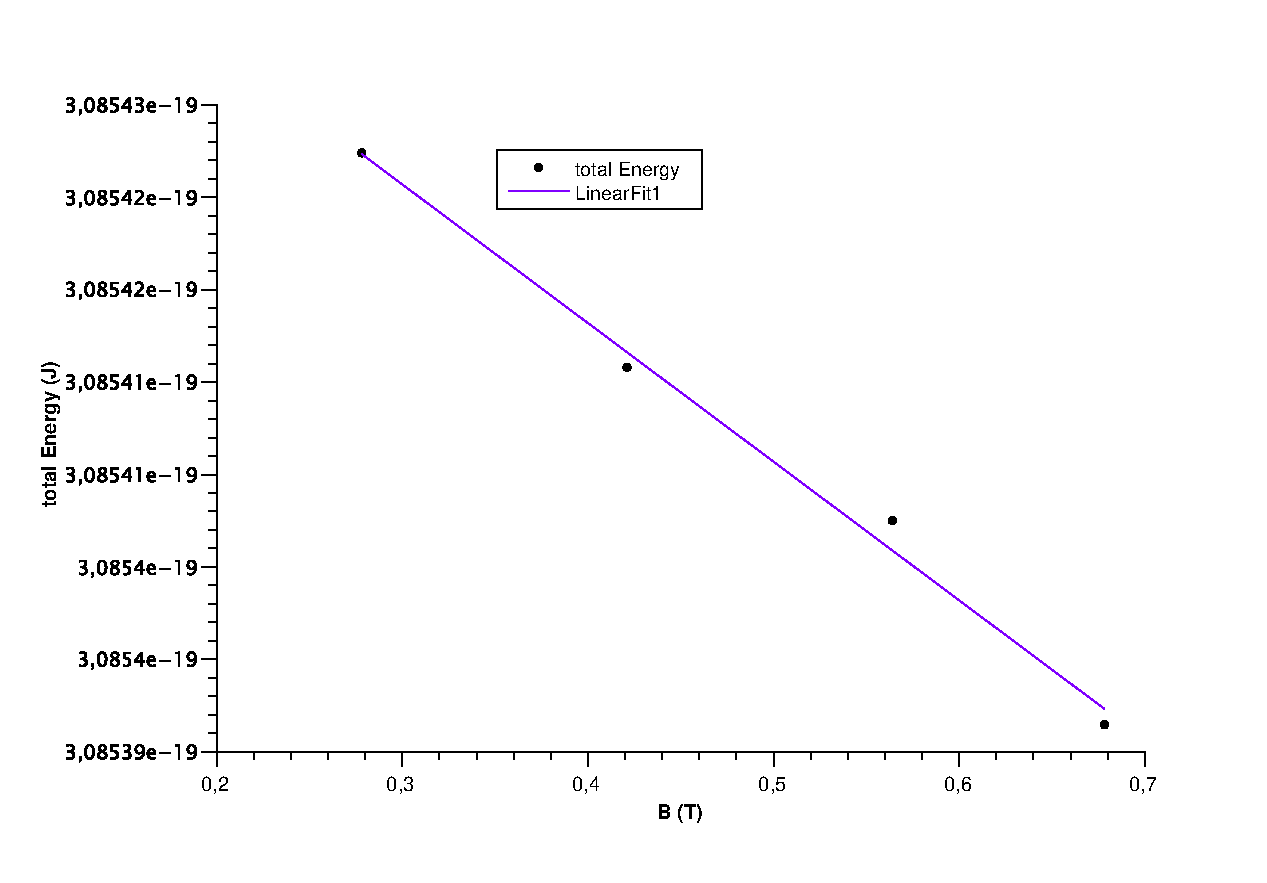
\includegraphics[width=0.7\textwidth]{E_function_B.eps}
    \caption{The total energy E as a function of the magnetic field B}
    \label{fig:E(B)}
\end{figure}

When fitting our data with a linear fit, the slope $s$ of this fit is directly proportional to the value of the Bohr magneton: $\mu_B = -s$. We obtain the value: \begin{equation} \mu_{B,exp} = 7.502 \cdot 10^{-24} \ \text{J} \cdot \text{T}^{-1} \end{equation} This value deviates to the theoretical one by: \begin{equation} \frac{|\mu_{B,exp}-\mu_{B,theo}|}{\mu_{B,theo}} \approx 19.0 \% \end{equation}


\begin{figure}[h]
     \centering
     \begin{subfigure}[b]{0.3\textwidth}
         \centering
         \includegraphics[width=\textwidth]{Polarizierung/1651244594804.jpg}
         \caption{Polarization at 0°} 
         \label{fig:pol0}
     \end{subfigure}
     \hfill
     \begin{subfigure}[b]{0.3\textwidth}
         \centering
         \includegraphics[width=\textwidth]{Polarizierung/1651244594819.jpg}
         \caption{Polarization at 90°}
         \label{fig:pol90}
     \end{subfigure}
     \hfill
     \begin{subfigure}[b]{0.3\textwidth}
         \centering
         \includegraphics[width=\textwidth]{Polarizierung/1651244594842.jpg}
         \caption{Polarization at 45°}
         \label{fig:pol45}
     \end{subfigure}
     \caption{Effect of the polarization angle on the spectral lines}
     \label{fig:polEffect}
\end{figure}
\FloatBarrier

A transversal configuration has been used to analyse the effects of polarization on the splitted spectral lines. As seen in the figures above, it is possible to filter out some lines with a linear polarizer.
When the polarization angle is at 0°, so the polarization filter is parallel to the magnetic field, then the spectral lines are the same as as when observed without B-field. Then 3 splitted lines are visible for 45° and occure due to the Zeeman effect. Finally, we get 2 splitted lines for 90°.
The longitudinal configuration, by rotating the electromagnet by 90°, wasn't working for us, since we should see two lines that stay unchanged regarding the polarization angle. We could see either one or two lines.

\section{Conclusion}
In this lab course, we discovered the effects on the spectral lines of a Cadmium lamp when introduced in a magnetic field. We could see that the lines split in function of \dots. By measuring the distance of the change in the aperture angle $\delta \alpha$ and the change of aperture angle between two interference orders $\Delta \alpha$, the Bohr magneton can be determined and results in $\mu_{B,exp} = 7.502 \cdot 10^{-24} \ \text{J} \cdot \text{T}^{-1}$, which corresponds to a relative error of 19.0 \%. Then, for the analysis of the polarization on the Zeeman effect, we saw that the light of the three rings in a transversal configuration is linearly polarized.

\section{Appendix}
\textbf{Derivation of equation \ref{equation_delta_lambda}:}
For this part we try to establish a relation between the change in the wavelength $\delta \lambda$ and $\delta \alpha$ and $\Delta \alpha$. To do this, first we need to solve for $\alpha$ using equation 23 from the handout \cite{Handout}:
\begin{align}
    \Delta &= 2d\cdot \sqrt{n^2 -\sin{\alpha}^2} = k\lambda \\
    \sin{\alpha}^2 &= n^2-\left(\frac{k\lambda}{2d}\right)^2\\
    \alpha &= \arcsin{\sqrt{n^2-\left(\frac{k\lambda}{2d}\right)^2}}
\end{align}

Now, taking the derivative with respect to $\lambda$, knowing that the derivative of $\arcsin{x}$ is $\sqrt{\frac{1}{1-x^2}}$ with x being $n^2-\left(\frac{k\lambda}{2d}\right)^2$.

\begin{equation}
    \frac{\delta \alpha}{\delta \lambda} = {\frac{-k^2\lambda}{\sqrt{1-n^2+\left(\frac{k\lambda}{2d}\right)^2}}}
    \label{equation_delta}
\end{equation}

The same can be done with respect to k:

\begin{equation}
    \frac{\Delta \alpha}{\Delta k} = {\frac{-\lambda^2k}{\sqrt{1-n^2+\left(\frac{k\lambda}{2d}\right)^2}}}
    \label{equation_Delta}
\end{equation}

Now dividing equation \ref{equation_Delta} with equation \ref{equation_delta}, we get:

\begin{align}
    \frac{\Delta\alpha \delta \lambda}{\Delta k \delta \alpha} &= \frac{\lambda^2k}{k^2\lambda} \\
    \frac{\Delta\alpha \delta \lambda}{\Delta k \delta \alpha} &= \frac{\lambda}{k}\\
    \delta \lambda = \frac{\lambda \Delta k}{k} &\cdot \frac{\delta \alpha}{\Delta \alpha}
\end{align}

Since k are integer steps, its derivative $\Delta k$ is 1.
Using equation 9, we get an expression for k :
\begin{equation}
    k = \frac{2d\cdot \sqrt{n^2 -\sin{\alpha}^2}}{\lambda}
\end{equation}

Finally, plugging k into equation 16 we get the final result:
\begin{equation}
    \delta \lambda = \frac{\lambda^2}{2d\cdot \sqrt{n^2 -\sin{\alpha}^2}} \cdot \frac{\delta \alpha}{\Delta \alpha}
\end{equation}



\begin{thebibliography}{}
\bibitem{Tipler} \textit{Modern Physics}, Paul A. Tipler and Ralph A. Llewellyn, (sixth edition, 2012)
 \bibitem{Handout} Handout from the supervisor: \textit{Magnetic properties of atoms} (version 1.2)
 \bibitem{Zeeman} \textit{Zeeman effect}, Wikipedia, \url{https://en.wikipedia.org/wiki/Zeeman_effect}(last visited 21/05/2022)
\end{thebibliography}

\end{document}
